\documentclass[11pt,a4paper]{article}

\usepackage{graphicx}
\title{Interfacing ADC with R-PI}
\author{e-Yantra Team}
\date{\today}

\begin{document}
	\maketitle
	\newpage
	\tableofcontents
	\newpage
	
\section{Objective}
The objective is to Interface the ADC MCP3008 to Raspberry Pi with a Sharp IR Sensor as Raspberry Pi has no built in analogue inputs which means it is a bit of a pain to use many of the available sensors.
	\section{Prerequisites}
	One should have:
	\begin{itemize}
		\item To know how to access the pins of an R-Pi.
		\item Some basic information regarding SPI protocol.
        \item Python programming skills.
	\end{itemize}
	
	\section{Hardware Requirement}
	\begin{enumerate}
		\item Raspberry Pi (I will be using Version 2 Model B)
		\item Power adapter(5V)
		\item MCP3008
        \item Sharp IR Sensor
        \item White Line Sensor
		\item Connecting wires
		\item Bread board
	\end{enumerate}
	
	
	\section{Software Requirement}
	\begin{enumerate}
	 \item MobaXterm (for windows user)
	 \item PyScripter (version 2.7 or above)
    \end{enumerate}
	
	\section{Theory and Description}
	
		
	   \subsection{MCP 3008}
    \begin{figure}[h!]
		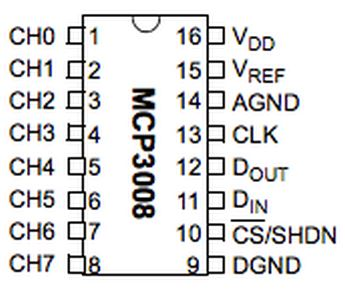
\includegraphics[scale=0.7]{mcp.jpg}
		\centering
		\caption{MCP3008}
	    \end{figure}

\begin{itemize}
\item The MCP3008 is a 10bit 8-channel Analogue-to-digital converter (ADC).[1]
\item It is cheap, easy to connect and doesn�t require any additional components.
\item It uses the SPI bus protocol which is supported by the Pi�s GPIO header.

\item The experiment explains how to use an MCP3008 [5] device to provide 8 analogue inputs which you can use with a range of sensors.
     \item In the circuit I use my MCP3008 to read a Sharp IR sensor.
\end{itemize}

	\subsection{SPI}
\begin{itemize}
\item The Serial Peripheral Interface (SPI) is a communication protocol used to transfer data between micro-computers like the Raspberry Pi and peripheral devices.[2]
    \item These peripheral devices may be either sensors or actuators.
    \item In this example, we will be learning to use an Analog to Digital Converter (ADC) sensor.
    \item An analog to digital sensor takes an analog voltage and converts it into a digital number that can be understood by the Raspberry Pi.
\end{itemize}


SPI uses 4 separate connections to communicate with the target device. These connections are:
\begin{enumerate}
\item Serial clock (CLK)
\item Master Input Slave Output (MISO)
\item Master Output Slave Input (MOSI) and
\item Chip Select (CS).
\end{enumerate}

\begin{itemize}
	\item The \textbf{Clock pin} sense pulses at a regular frequency, the speed at which the Raspberry Pi and SPI device agree to transfer data to each other. For the ADC, clock pulses are sampled on their rising edge, on the transition from low to high.\\
\item The \textbf{MISO }pin is a data pin used for the master (in this case the Raspberry Pi) to receive data from the ADC. Data is read from the bus after every clock pulse.[3]\\
\item The \textbf{MOSI} pin sends data from the Raspberry Pi to the ADC. The ADC will take the value of the bus on the rising edge of the clock. This means the value must be set before the clock is pulsed.\\
\item Finally, the \textbf{Chip Select line} chooses which particular SPI device is in use. If there are multiple SPI devices, they can all share the same CLK, MOSI, and MISO. However, only the selected device has the Chip Select line set low, while all other devices have their CS lines set high. A high Chip Select line tells the SPI device to ignore all of the commands and traffic on the rest of the bus.\\
\end{itemize}


\newpage	
\section{Experiment}
\subsection{Interfacing an ADC with RPi using a Sharp IR Sensor}
        \begin{figure}[h!]
		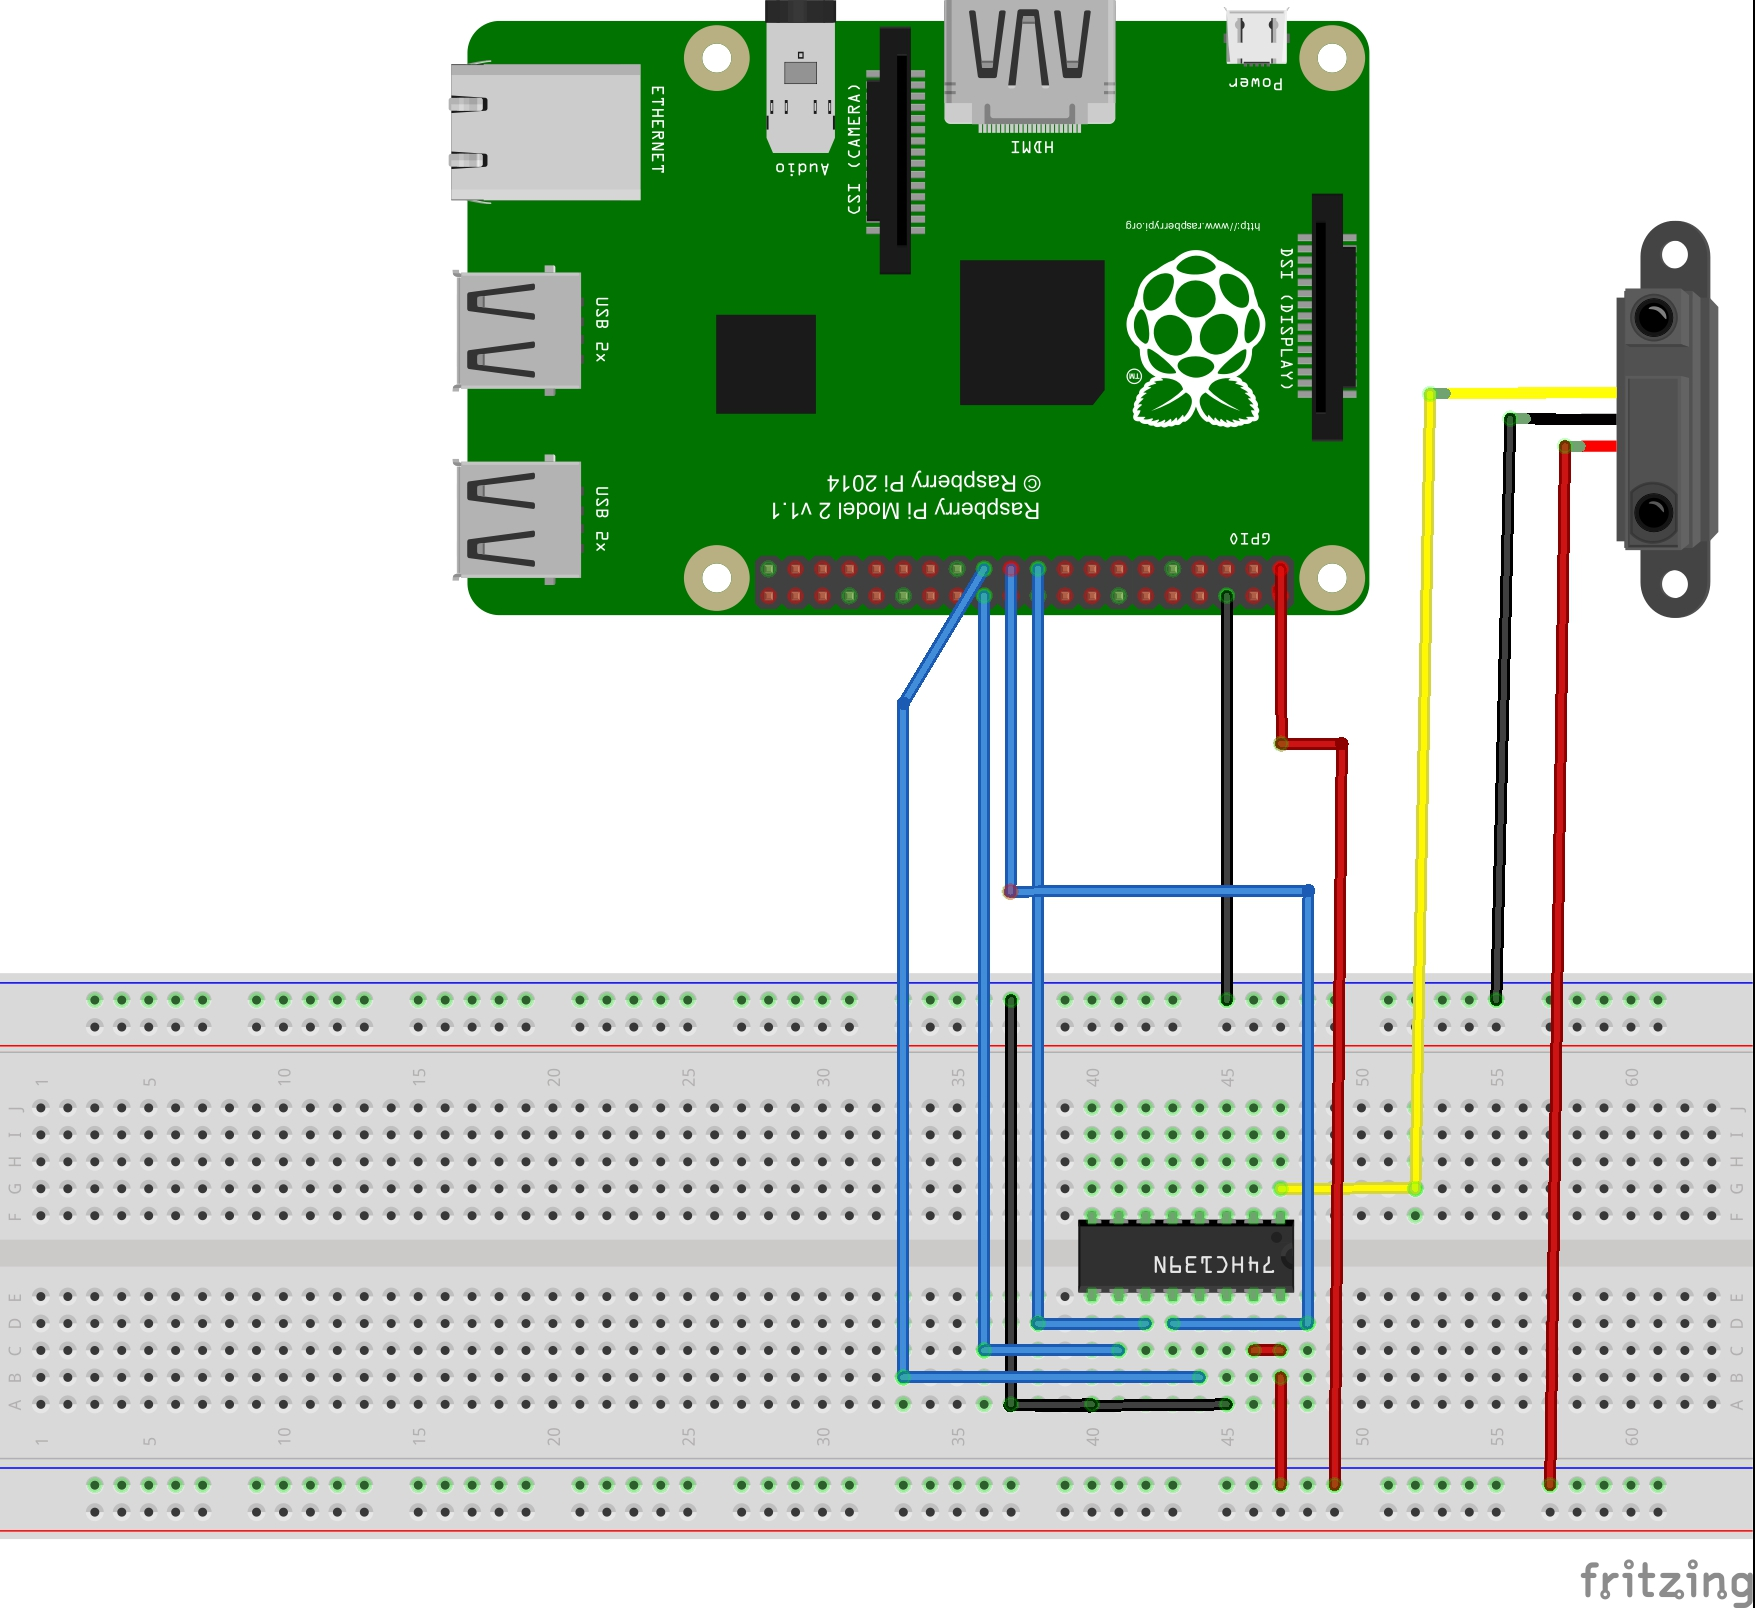
\includegraphics[scale=0.7]{ckt.jpg}
		\centering
        \caption{Circuit on Bread Board}
        \end{figure}
  \begin{itemize}
  \item The pin connections are shown in the Circuit above.
  \item The Connections are showed in the Circuit Schematic in the next figure.
  \item Here I have used a single ADC MCP3008 interfaced with RPi to which a Sharp IR Sensor is connected.
  \item In the next Experiment I will use 2 ADC's which will be interfaced with RPi using the 2 chip select pins CE0 and CE1.
  \end{itemize}

\newpage
\subsection{Circuit Schematic}
        \vspace{3cm}
        \begin{figure}[h!]
		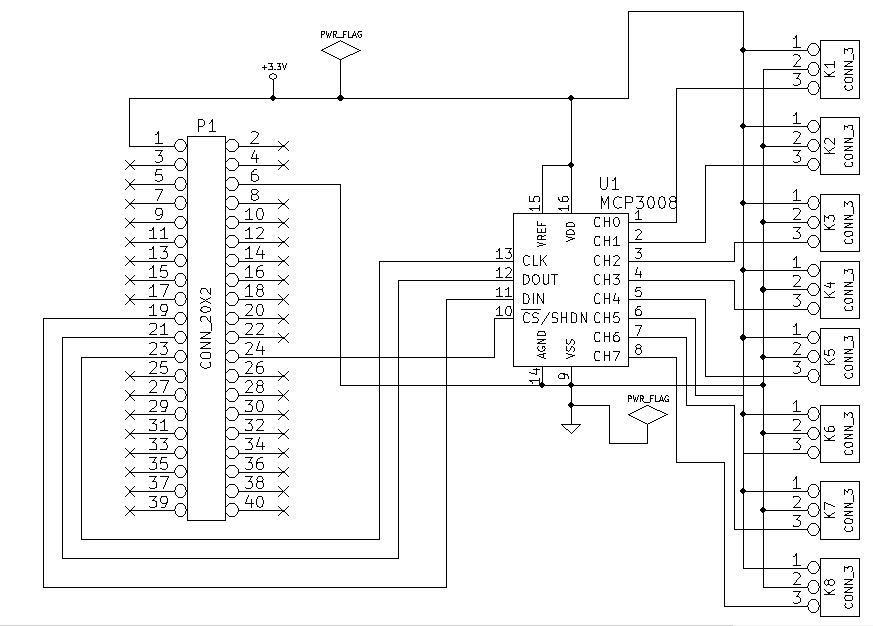
\includegraphics[scale=0.6]{ckt_schematic.jpg}
		\centering
        \caption{Circuit Schematic}
        \end{figure}
\newpage
\subsection{Code}

\begin{verbatim}
import os
import spidev
import time

# Open SPI bus[4]
spi = spidev.SpiDev()#  to create spi object
spi.open(0,0)#Clock polarity,Clock Phase

# Function to read SPI data from MCP3008 chip
# Channel must be an integer 0-7
def ReadChannel(channel):
#Performs SPI Transaction and CS will be held active
  adc = spi.xfer2([1,(8+channel)<<4,0])
  data = ((adc[1]&3) << 8) + adc[2]
  return data

# Function to convert data to voltage level,
# rounded to specified number of decimal places.
def ConvertVolts(data,places):
  volts = (data * 3.3) / float(1023)
  volts = round(volts,places)
  return volts


# This Function calculates the actual distance in millimeters(mm) from the input
# analog value of Sharp Sensor.
def Sharp_GP2D12_estimation(adc_reading):

	
		  distance =(10.00*(2799.6*(1.00/(pow(adc_reading,1.1546)))))
		  distanceInt = distance
		  if distanceInt>800:
	
		  	distanceInt=800
	
	      return distanceInt

# Define sensor channels
sharp_channel =0


# Define delay between readings
delay =0.5

try:
      while True:

			# Read the sharp sensor data
			sharp_level = ReadChannel(sharp_channel)
			sharp_volts = ConvertVolts(sharp_level,3)
			value = Sharp_GP2D12_estimation(sharp_level)


			# Print out results
			print "--------------------------------------------"
			print("sharp: Digital {} (Analog {}V)".format(sharp_level,sharp_volts))
			print("sharp:  (Distance {} cm)".format(value))

			# Wait before repeating loop
			time.sleep(delay)


except KeyboardInterrupt:
       pass

\end{verbatim}


\newpage
\subsection{PCB Designing}
        \begin{figure}[h!]
		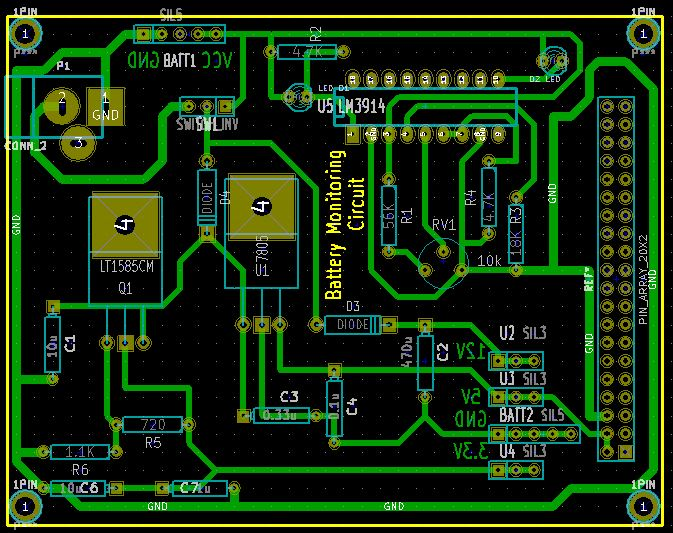
\includegraphics[scale=1]{pcb.jpg}
		\centering
        \caption{PCB}
        \end{figure}

\newpage	
\section{Exercise}
\subsection{Interfacing 2 ADC's with RPi using a Sharp IR and White line sensor}
\begin{itemize}
  \item The pin connections are shown in the Circuit Schematic.
  \item Here I have used 2 MCP3008 ADC's interfaced with RPi.
  \item In the this experiment I have used Sharp IR Sensor and White line sensor.
  \item 2 ADC's can be interfaced with RPi mainly because of the 2 chip select pins CE0 and CE1 in RPi.
  \end{itemize}
  \subsection{Circuit Schematic}
        \begin{figure}[h!]
		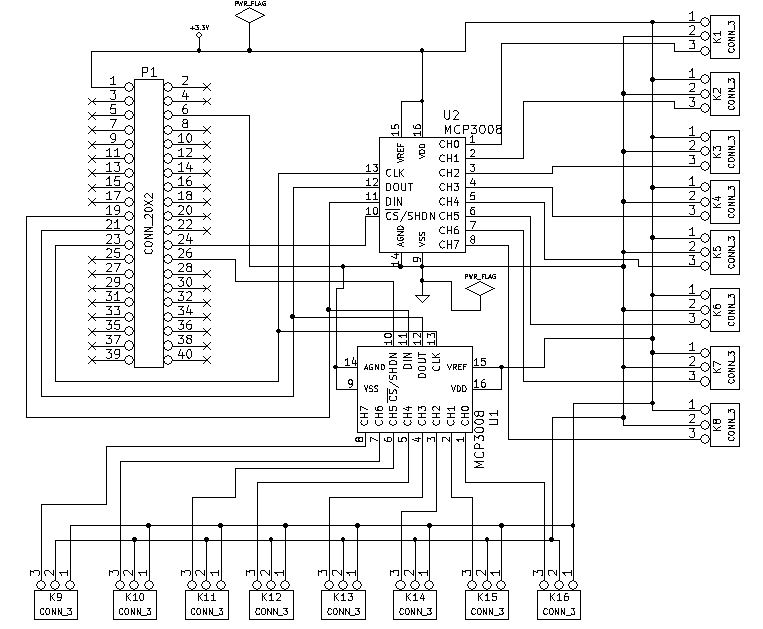
\includegraphics[scale=0.6]{ckt_schematic2.jpg}
		\centering
        \caption{Circuit Schematic}
        \end{figure}
\newpage
\subsection{Code}

\begin{verbatim}
import os
import spidev # module to control spi devices
import time
import RPi .GPIO as GPIO # module to control Pi GPIO channels


# Open SPI bus
spi = spidev.SpiDev()#  to create spi object
spi.open(0,0)#Clock polarity,Clock Phase

# Function to read SPI data from MCP3008 chip
# Channel must be an integer 0-7
def ReadChannel(channel):
#Performs SPI Transaction and CS will be held active
  adc = spi.xfer2([1,(8+channel)<<4,0])
  data = ((adc[1]&3) << 8)
  return data

# Function to convert data to voltage level,
# rounded to specified number of decimal places.
def ConvertVolts(data,places):
  volts = (data * 3.3) / float(1023)
  volts = round(volts,places)
  return volts


# This Function calculates the actual distance in millimeters(mm) from the input
# analog value of Sharp Sensor.
def Sharp_GP2D12_estimation(adc_reading):

	
		  distance =(10.00*(2799.6*(1.00/(pow(adc_reading,1.1546)))))
		  distanceInt = distance
		  if distanceInt>800:
	
		  	distanceInt=800
	
	          return distanceInt
# Define sensor channels
sharp_channel =0
white_channel =1

# Define delay between readings
delay =0.5

try:
      while True:
            GPIO.setmode(GPIO.BOARD)
            # set up GPIO output channel
            GPIO.setup(24, GPIO.OUT)
            GPIO.setup(26, GPIO.OUT)

            GPIO.output(24,GPIO.LOW)
            GPIO.output(26,GPIO.HIGH)

			# Read the sharp sensor data
			sharp_level = ReadChannel(sharp_channel)
			sharp_volts = ConvertVolts(sharp_level,3)
			value = Sharp_GP2D12_estimation(sharp_level)

            GPIO.output(26,GPIO.LOW)
            GPIO.output(24,GPIO.HIGH)

			white_level=ReadChannel(white_channel)
			white_volts = ConvertVolts(white_level,3)
			
            # Print out results
			print "--------------------------------------------"
			print("sharp: Digital {} (Analog {}V)".format(sharp_level,sharp_volts))
			print("sharp:  (Distance {} cm)".format(value))

			print "--------------------------------------------"
			print("white: Digital {} (Analog {}V)".format(white_level,white_volts))
			
            # Wait before repeating loop
			time.sleep(delay)
        except KeyboardInterrupt:
       pass
\end{verbatim}


\newpage
\subsection{PCB Designing}
        \begin{figure}[h!]
		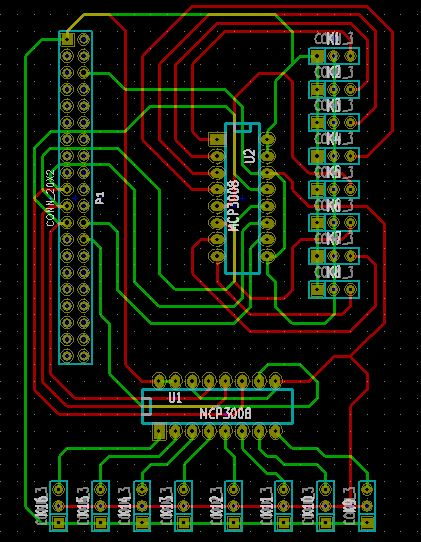
\includegraphics[scale=1]{pcb2.jpg}
		\centering
        \caption{PCB}
        \end{figure}

\newpage
		\section{References}
		\begin{enumerate}
			\item www.raspberrypi-spy.co.ukanalogue-sensors-on-the-raspberry-pi-using-an-mcp3008/
			\item www.en.wikipedia.org/wiki/SerialPeripheralInterface
			\item www.byteparadigm.com/applications/introduction-to-i2c-and-spi-protocols/
			\item developers.google.com/edu/python/
            \item www.alldatasheet.com/Mcp3008+datasheet
		\end{enumerate}	
	
	


\end{document}



